\section{Experimental Evaluation}
\label{sec:results}
In this section, we first describe the datasets and the evaluation setting for our experiments (\cref{sec:dataset_evalsetting}). We then proceed with a quantitative evaluation of our method and showcase its applicability to downstream tasks with qualitative results for surface reconstruction~(\cref{sec:evaluation_results}). Finally, we validate our design choices in an ablation study~(\cref{sec:ablation}).

\subsection{Datasets and evaluation setting}
\label{sec:dataset_evalsetting}

\paragraph{Waymo} The Waymo Open Dataset~\cite{sun2020scalability} includes 798/202 scenes for training/validation, where each scene is a 20-second clip captured by a 64-beam LiDAR at 10~Hz. We randomly sample 573/201 scenes for training/validation from the training split, and treat the whole validation split as a held-out test set. We consider every 5 consecutive frames as a \textit{sample} and extract 20 \textit{samples} from each clip, for a total of 11440/4013/4031 samples for training/validation/test. %
    
\paragraph{nuScenes} The nuScenes dataset~\cite{caesar2020nuscenes} consists of 700 training and 150 validation scenes, where each scene is a 20-second clip captured by a 32-beam LiDAR at 20$\,$Hz. We use all validation scenes for testing and randomly hold out 150 training scenes for validation. We consider every 11 consecutive frames as a \textit{sample}, resulting in a total of 10921/2973/2973 samples for training/validation/testing.

\paragraph{Ground truth} We follow~\cite{jund2021scalable} to construct pseudo ground-truth from the detection and tracking annotations. Specifically, the flow vectors of the background part are obtained from ground truth ego-motion. For foreground objects, we use the
unique instance IDs of the tracking annotations and recover their rigid motion parameters by registering the bounding boxes.
Notably, for \nuscenes~the bounding boxes are only annotated every 10 frames. To obtain pseudo ground truth for the remaining frames, we linearly interpolate the boxes, which may introduce a small amount of label noise especially for fast-moving objects.

\begin{table}[t]
    \setlength{\tabcolsep}{6pt}
    \renewcommand{\arraystretch}{1.2}
	\centering
	\resizebox{\columnwidth}{!}{
    \begin{tabular}{clcccc|cccccc}
    \toprule
    & & \multicolumn{4}{c|}{Static part} & \multicolumn{5}{c}{Dynamic foreground}  \\
    Dataset                   & Method    & EPE avg.$\downarrow$ & AccS$\uparrow$  & AccR$\uparrow$ & ROutlier$\downarrow$ & EPE avg. $\downarrow$ & EPE med.$\downarrow$  & AccS$\uparrow$   & AccR$\uparrow$   & ROutliers $\downarrow$                 \\
    \midrule
    \multirow{7}{*}{\emph{Waymo}}    & PPWC-Net~\cite{wu2019pointpwc}  & 0.414 & 17.6 & 40.2 & 12.1 & 0.475 & 0.201 & 9.0 & 29.3 & 22.4  \\
                              & FLOT~\cite{puy2020flot} & 0.129 & 65.2 & 85.0 & 2.8 & 0.625 & 0.231 & 9.8 & 27.4 & 33.8   \\
                              & WsRSF~\cite{gojcic2021weakly} & 0.063 & 87.3 & 96.6 & 0.6 & 0.381 & 0.094 & 31.3 & 64.0 & 10.1       \\
                              & NSFPrior~\cite{li2021neural} & 0.187 & 79.8 & 89.1 & 4.7 & 0.237 & 0.077 & 44.7 & 68.6 & 11.5\\                     \arrayrulecolor{lightgray}\cline{2-11}\arrayrulecolor{black}
                              & Ours & \underline{0.028} & \underline{97.5} & \underline{99.5} & \underline{0.1} & \underline{0.197} & \underline{0.062} & \underline{53.3} & \underline{77.5} & \underline{5.9}  \\
                              & Ours+ & \textbf{0.018} & \textbf{99.0} & \textbf{99.7} & \textbf{0.1} & \textbf{0.173} & \textbf{0.043} & \textbf{69.1} & \textbf{86.9} & \textbf{5.1} \\
                              & Ours (w.\ ground) & 0.042 & 91.9 & 98.8 & 0.1 & 0.219 & 0.071 & 47.1 & 72.8 & 8.5 \\            
    \midrule
    \multirow{7}{*}{\emph{nuScenes}} & PPWC-Net~\cite{wu2019pointpwc}  & 0.316 & 16.1 & 37.0 & 8.7 & 0.661 & 0.307 & 7.6 & 24.2 & 31.9\\
                                  & FLOT~\cite{puy2020flot} & 0.153 & 51.7 & 78.3 & 4.3 & 1.216 & 0.710 & 3.0 & 10.3 & 63.9 \\
                                  & WsRSF~\cite{gojcic2021weakly} & 0.195 & 57.4 & 82.6 & 4.8 & 0.539 & 0.204 & 17.9 & 37.4 & 22.9 \\
                                  & NSFPrior~\cite{li2021neural} &  0.584 & 38.9 & 56.7 & 26.9 & 0.707 & 0.222 & 19.3 & 37.8 & 32.0 \\
                                  \arrayrulecolor{lightgray}\cline{2-11}\arrayrulecolor{black}
                                  & Ours & \underline{0.111} & \underline{65.4} & \underline{88.6} & \underline{1.1} & \underline{0.301} & \underline{0.146} & \underline{26.6} & \underline{53.4} & \textbf{12.1} \\
                                  & Ours+ & \textbf{0.091} & \textbf{72.8} & \textbf{91.9} & \textbf{0.9} & \textbf{0.301} & \textbf{0.135} & \textbf{32.7} & \textbf{56.7} & \underline{13.7} \\
                                  & Ours (w.\ ground) & 0.134 & 55.3 & 83.8 & 1.9 & 0.37 & 0.182 & 18.2 & 43.8 & 17.5  \\   
    \bottomrule
    \end{tabular}
    }
	\caption{Scene flow results on \emph{Waymo} and \emph{nuScenes} datasets.}
	\label{tab:sf_main}
\end{table}
\paragraph{Metrics}
We use standard \emph{scene flow} evaluation metrics~\cite{liu2019flownet3d,baur2021slim} to compare the performance of our approach to the selected baselines. These metric include:
\textit{(i)} 3D end-point-error~(\textit{EPE}~[m]) which denotes the mean $L_2$-error of all flow vectors averaged over all frames; 
\textit{(ii)} strict/relaxed accuracy (\textit{AccS}~[\%]~/\textit{AccR}~[\%]). \ie, the fraction of points with \textit{EPE} $<$ 0.05/0.10m or relative error $<$ 0.05/0.10; \textit{(iii)} \textit{Outliers~[\%]} which denotes the ratio of points with \textit{EPE} $>$ 0.30m or relative error $>$ 0.10; and \textit{(iv)} \textit{ROutliers}~[\%], the fraction of points whose \textit{EPE} $>$ 0.30m and relative error $>$ 0.30. We evaluate these metrics for the static and dynamic parts of the scene separately.\footnote{A point is labelled as \textit{dynamic} if its ground-truth velocity is $>0.5\,$m/s.} %
Following \cite{wu2020motionnet,luo2021self}, we evaluate the performance of all methods only on the points that lie within the square of size $64\times 64$ m$^2$ centered at the ego-car location in the target frame. Additionally we remove ground points by thresholding along the $z$-axis.\footnote{This setting turns out to better suit the baseline methods~\cite{puy2020flot,wu2019pointpwc,li2021neural}. However, we keep ground points in our dynamic point cloud accumulation task, as thresholding could falsely remove points that are of interest for reconstruction or mapping.} Ablations studies additionally report the quality of \textit{motion segmentation} in terms of recall and precision of \textit{dynamic} parts, and the quality of \textit{spatio-temporal instance association} in terms of mean weighted coverage (\textit{mWCov}, the \textit{IoU} of recovered instances~\cite{wang2019associatively}). For further details, see the appendix.

\paragraph{Baselines}
We compare our method to 4 baseline methods. PPWC~\cite{wu2019pointpwc} and FLOT~\cite{puy2020flot} are based on dense matching and are trained in a fully supervised manner; WsRSF~\cite{gojcic2021weakly} assumes a \textit{multi-body} scene and can be trained with weak supervision; NSFPrior~\cite{li2021neural} is an optimisation-based method without pre-training. For PPWC~\cite{wu2019pointpwc}, FLOT~\cite{puy2020flot} and WsRSF~\cite{gojcic2021weakly}, we sample at most 8192 points from each frame due to memory constraints, and use the $k$-nn graph to up-sample flow vectors to full resolution at inference time. For NSFPrior~\cite{li2021neural}, we use the full point clouds and take the default hyper-parameter settings given by the authors, except for the early-stopping patience, which we set to 50 to make it computationally tractable on our large-scale dataset. For all baseline methods, we directly estimate flow vectors from any \textit{source} frame to the \textit{target} frame. 

\subsection{Main results}
\label{sec:evaluation_results}
The detailed comparison on the \waymo~and \nuscenes~data is given in \cref{tab:sf_main}. \emph{Ours} denotes the direct output of our model, while \emph{Ours+} describes the results after test-time refinement with ICP. Many downstream tasks (e.g., surface reconstruction) rely on the accumulation of full point clouds and require also ground points. We therefore also train a variant of our method on point clouds with ground points and denote it \emph{Ours (w. ground)}. To facilitate a fair comparison, we use full point clouds as input during training and inference, but only compute the evaluation metrics on points that do not belong to ground. 

\paragraph{Comparison to state of the art}
\begin{figure}[t!]
    \centering
    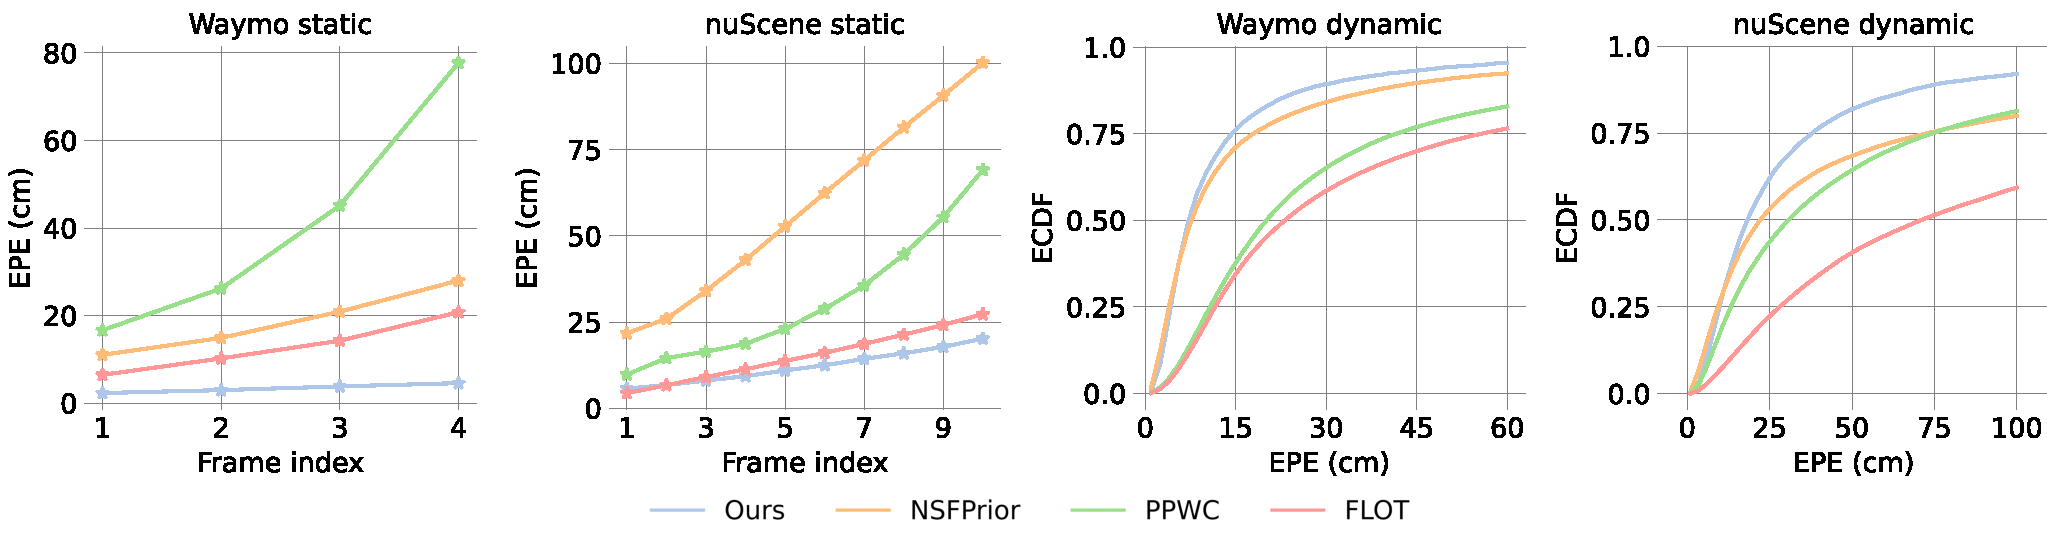
\includegraphics[width=1.0\columnwidth]{figs/figure/figure_1.pdf}
    \caption{Our method scales better to more frames. For the challenging dynamic parts, it also has smaller errors as well as fewer extreme outliers.}
    \label{fig:epe3d_ecdf}
\end{figure}
On the static part of the \textbf{\waymo}~dataset, FLOT~\cite{puy2020flot} reaches the best performance among the baselines, but still has an average EPE error of 12.9$\,$cm, which is more than 4 times larger than that of \textit{Ours} (2.8$\,$cm). This result corroborates our motivation for decomposing the scene into a static background and dynamic foreground. Modeling the motion of the background with a single set of transformation parameters also enables us to run ICP at test time (\textit{Ours+}), which further reduces the EPE of the static part to 1.8$\,$cm. On the dynamic foreground points, NSFPrior~\cite{li2021neural} reaches a comparable performance to \textit{Ours}. However, based on our spatio-temporal association of foreground points we can again run ICP at test-time, which reduces the median EPE error to 4.3$\,$cm, $\approx$40$\,\%$ lower than that of NSFPrior. Furthermore, NSFPrior is an optimization method and not amenable to online processing (see Tab.~\ref{tab:runtime}). The results for \textbf{\nuscenes} follow a similar trend as the ones for \emph{Waymo}, but are larger in absolute terms due to the lower point density. Our method achieves the best performance on both static and dynamic parts. The gap to the closest competitors is even larger, which auggests that our method is more robust to low point density.

To further understand the error distribution of the dynamic parts, and the evolution of the errors of the static part as the gap between the \textit{source} and \textit{target} frames increases, we plot detailed results in \cref{fig:epe3d_ecdf}. On both \waymo~and \nuscenes{} our method degrades gracefully, and slower than the baselines. The ECDF curve of the EPE error for foreground points also shows that our method performs best at all thresholds. 

\paragraph{Breakdown of the performance gain}
Overall, our method improves over baseline methods by a large margin on two datasets. The gains are a direct result of our design choices: \textit{(i)}~by modelling the flow of the background as rigid motion instead of unconstrained flow, we can greatly reduce \emph{ROutlier} and improve the accuracy; \textit{(ii)}~different from~\cite{gojcic2021weakly} we perform motion segmentation, and can thus assign ego-motion flow to points on movable, but \emph{static} objects ($\approx75\%$ of the foreground). This further improves the results (see EPE of static FG in \cref{tab:ablations}); \textit{(iii)}~reasoning on the object level, combined with spatio-temporal association and modelling, improves flow estimates for the \textit{dynamic} foreground.

\paragraph{Generalisation to variable input length $T$}
\label{sec: more frames}
When trained with a fixed input length ($T=5$ on \emph{Waymo}), our model is able to generalize to different input lengths (see Tab.~\ref{tab:generalisation}). The performance degrades moderately with increasing $T$, as the motions become larger than seen during training. Also, larger displacements make the correspondence problem inherently harder.
\begin{table}[t]
    \setlength{\tabcolsep}{6pt}
    \renewcommand{\arraystretch}{1.2}
	\centering
	\resizebox{0.7\columnwidth}{!}{
    \begin{tabular}{c|cccccccc}
    \toprule
    & 3 & 4 & 5 & 6 & 7 & 8 & 9 & 10 \\
    \midrule
    static EPE avg. & \textbf{0.022} & 0.025 & 0.028 & 0.032 & 0.037 & 0.044 & 0.054 & 0.066\\
    dynamic EPE avg. & 0.199 & \textbf{0.168} & 0.190 & 0.218 & 0.250 & 0.294 & 0.348 & 0.412 \\
    \bottomrule
    \end{tabular}
    }
    \caption{Scene flow results on \emph{Waymo} dataset w.r.t. input length.}
    \label{tab:generalisation}
\end{table}

% \begin{table}[t]
% 	\centering
% 	\begin{subfigure}[t]{0.3\columnwidth}
% 	    \vskip 0em
% 		\centering
% 		\resizebox{\textwidth}{!}{%
% 			\begin{tabular}{ccc}
%             \toprule
%                             & \emph{Waymo} &\emph{nuScenes} \\
%             \midrule
%             PPWC-Net~\cite{wu2019pointpwc}       &    \phantom{21}\underline{0.608}       &  \phantom{6}\underline{0.990}   \\
%             FLOT~\cite{puy2020flot}         &      \phantom{21}1.028     &  \phantom{6}2.010   \\
%             WsRSF~\cite{gojcic2021weakly}            &     \phantom{21}1.252      &    \phantom{6}1.460 \\
%             NSFPrior~\cite{li2021neural}            &     212.256      &    63.460 \\
%             Ours &      \phantom{21}\textbf{0.174}     &  \phantom{6}\textbf{0.250}  \\
%             \bottomrule
%             \end{tabular}
% 		}
% 	\end{subfigure}
% 	\hspace{5mm}
% 	\begin{subfigure}[t]{0.34\columnwidth}
% 		\vskip 0em
% 		\centering
% 		\resizebox{\textwidth}{!}{%
% 			\begin{tabular}{ccc}
%             \toprule
%                             & \emph{Waymo} &\emph{nuScenes} \\
%             \midrule
%             ego-motion estimation & 0.100 & 0.188 \\
%             motion segmentation & 0.024 & 0.040 \\
%             instance association & 0.036 & 0.009 \\
%             TubeNet & 0.014 & 0.013\\
%             \bottomrule
%             \end{tabular}
% 		}
% 	\end{subfigure}
% 	\caption{Runtimes for the \waymo~and \nuscenes~datasets. All numbers are seconds per 5-frame (\emph{Waymo}), respectively 11-frame (\emph{nuScenes}) \textit{sample}.}
%  	\label{tab:runtime}
% \end{table}


% \begin{table}[t]
%     \centering
%     \begin{minipage}{0.45\textwidth}
%         \centering
%         \resizebox{\textwidth}{!}{%
%             \begin{tabular}{ccc}
%             \toprule
%                             & \emph{Waymo} &\emph{nuScenes} \\
%             \midrule
%             PPWC-Net~\cite{wu2019pointpwc}       &    \phantom{21}\underline{0.608}       &  \phantom{6}\underline{0.990}   \\
%             FLOT~\cite{puy2020flot}         &      \phantom{21}1.028     &  \phantom{6}2.010   \\
%             WsRSF~\cite{gojcic2021weakly}            &     \phantom{21}1.252      &    \phantom{6}1.460 \\
%             NSFPrior~\cite{li2021neural}            &     212.256      &    63.460 \\
%             Ours &      \phantom{21}\textbf{0.174}     &  \phantom{6}\textbf{0.250}  \\
%             \bottomrule
%             \end{tabular}
%         }
%     \end{minipage}%
%     \hspace{5mm}
%     \begin{minipage}{0.45\textwidth}
%         \centering
%         \resizebox{\textwidth}{!}{%
%             \begin{tabular}{ccc}
%             \toprule
%                             & \emph{Waymo} &\emph{nuScenes} \\
%             \midrule
%             ego-motion estimation & 0.100 & 0.188 \\
%             motion segmentation & 0.024 & 0.040 \\
%             instance association & 0.036 & 0.009 \\
%             TubeNet & 0.014 & 0.013\\
%             \bottomrule
%             \end{tabular}
%         }
%     \end{minipage}
%     \caption{Runtimes for the \waymo~and \nuscenes~datasets. All numbers are seconds per 5-frame (\emph{Waymo}), respectively 11-frame (\emph{nuScenes}) \textit{sample}.}
%     \label{tab:runtime}
% \end{table}


\begin{table}[t]
    \centering
    \makebox[\textwidth][c]{ % Center the box within the text width
        \begin{minipage}{0.4\textwidth}
            \centering
            \resizebox{\textwidth}{!}{%
                \begin{tabular}{ccc}
                \toprule
                                & \emph{Waymo} &\emph{nuScenes} \\
                \midrule
                PPWC-Net~\cite{wu2019pointpwc}       &    \phantom{21}\underline{0.608}       &  \phantom{6}\underline{0.990}   \\
                FLOT~\cite{puy2020flot}         &      \phantom{21}1.028     &  \phantom{6}2.010   \\
                WsRSF~\cite{gojcic2021weakly}            &     \phantom{21}1.252      &    \phantom{6}1.460 \\
                NSFPrior~\cite{li2021neural}            &     212.256      &    63.460 \\
                Ours &      \phantom{21}\textbf{0.174}     &  \phantom{6}\textbf{0.250}  \\
                \bottomrule
                \end{tabular}
            }
        \end{minipage}
        \hspace{5mm}
        \begin{minipage}{0.45\textwidth}
            \centering
            \resizebox{\textwidth}{!}{%
                \begin{tabular}{ccc}
                \toprule
                                & \emph{Waymo} &\emph{nuScenes} \\
                \midrule
                ego-motion estimation & 0.100 & 0.188 \\
                motion segmentation & 0.024 & 0.040 \\
                instance association & 0.036 & 0.009 \\
                TubeNet & 0.014 & 0.013\\
                \bottomrule
                \end{tabular}
            }
        \end{minipage}
    }
    \caption{Runtimes for the \waymo~and \nuscenes~datasets. All numbers are seconds per 5-frame (\emph{Waymo}), respectively 11-frame (\emph{nuScenes}) \textit{sample}.}
    \label{tab:runtime}
\end{table}
\paragraph{Runtime}
We report runtimes for our model and several baseline methods on both datasets in \cref{tab:runtime}~(left). Our method is significantly faster than all baselines under the multi-frame scene flow setting. We also report detailed runtimes of our model for individual steps in \cref{tab:runtime}~(right). As we can see, backbone feature extraction and pairwise registration (\textit{ego-motion estimation}) account for the majority of the runtime, 57.5\% on \waymo~and 75.2\% on \nuscenes. Note that this runtime is calculated over all frames, while under a data streaming setting, we only need to run the first part for a single incoming frame, then re-use the features of the previous frames at later stages, which will greatly reduce runtime: after initialisation, the runtime for every new sample decreases to around 0.094$\,$s for \waymo, respectively 0.079$\,$s on \nuscenes. 

\paragraph{Qualitative results}
\begin{figure}[t]
    \centering
    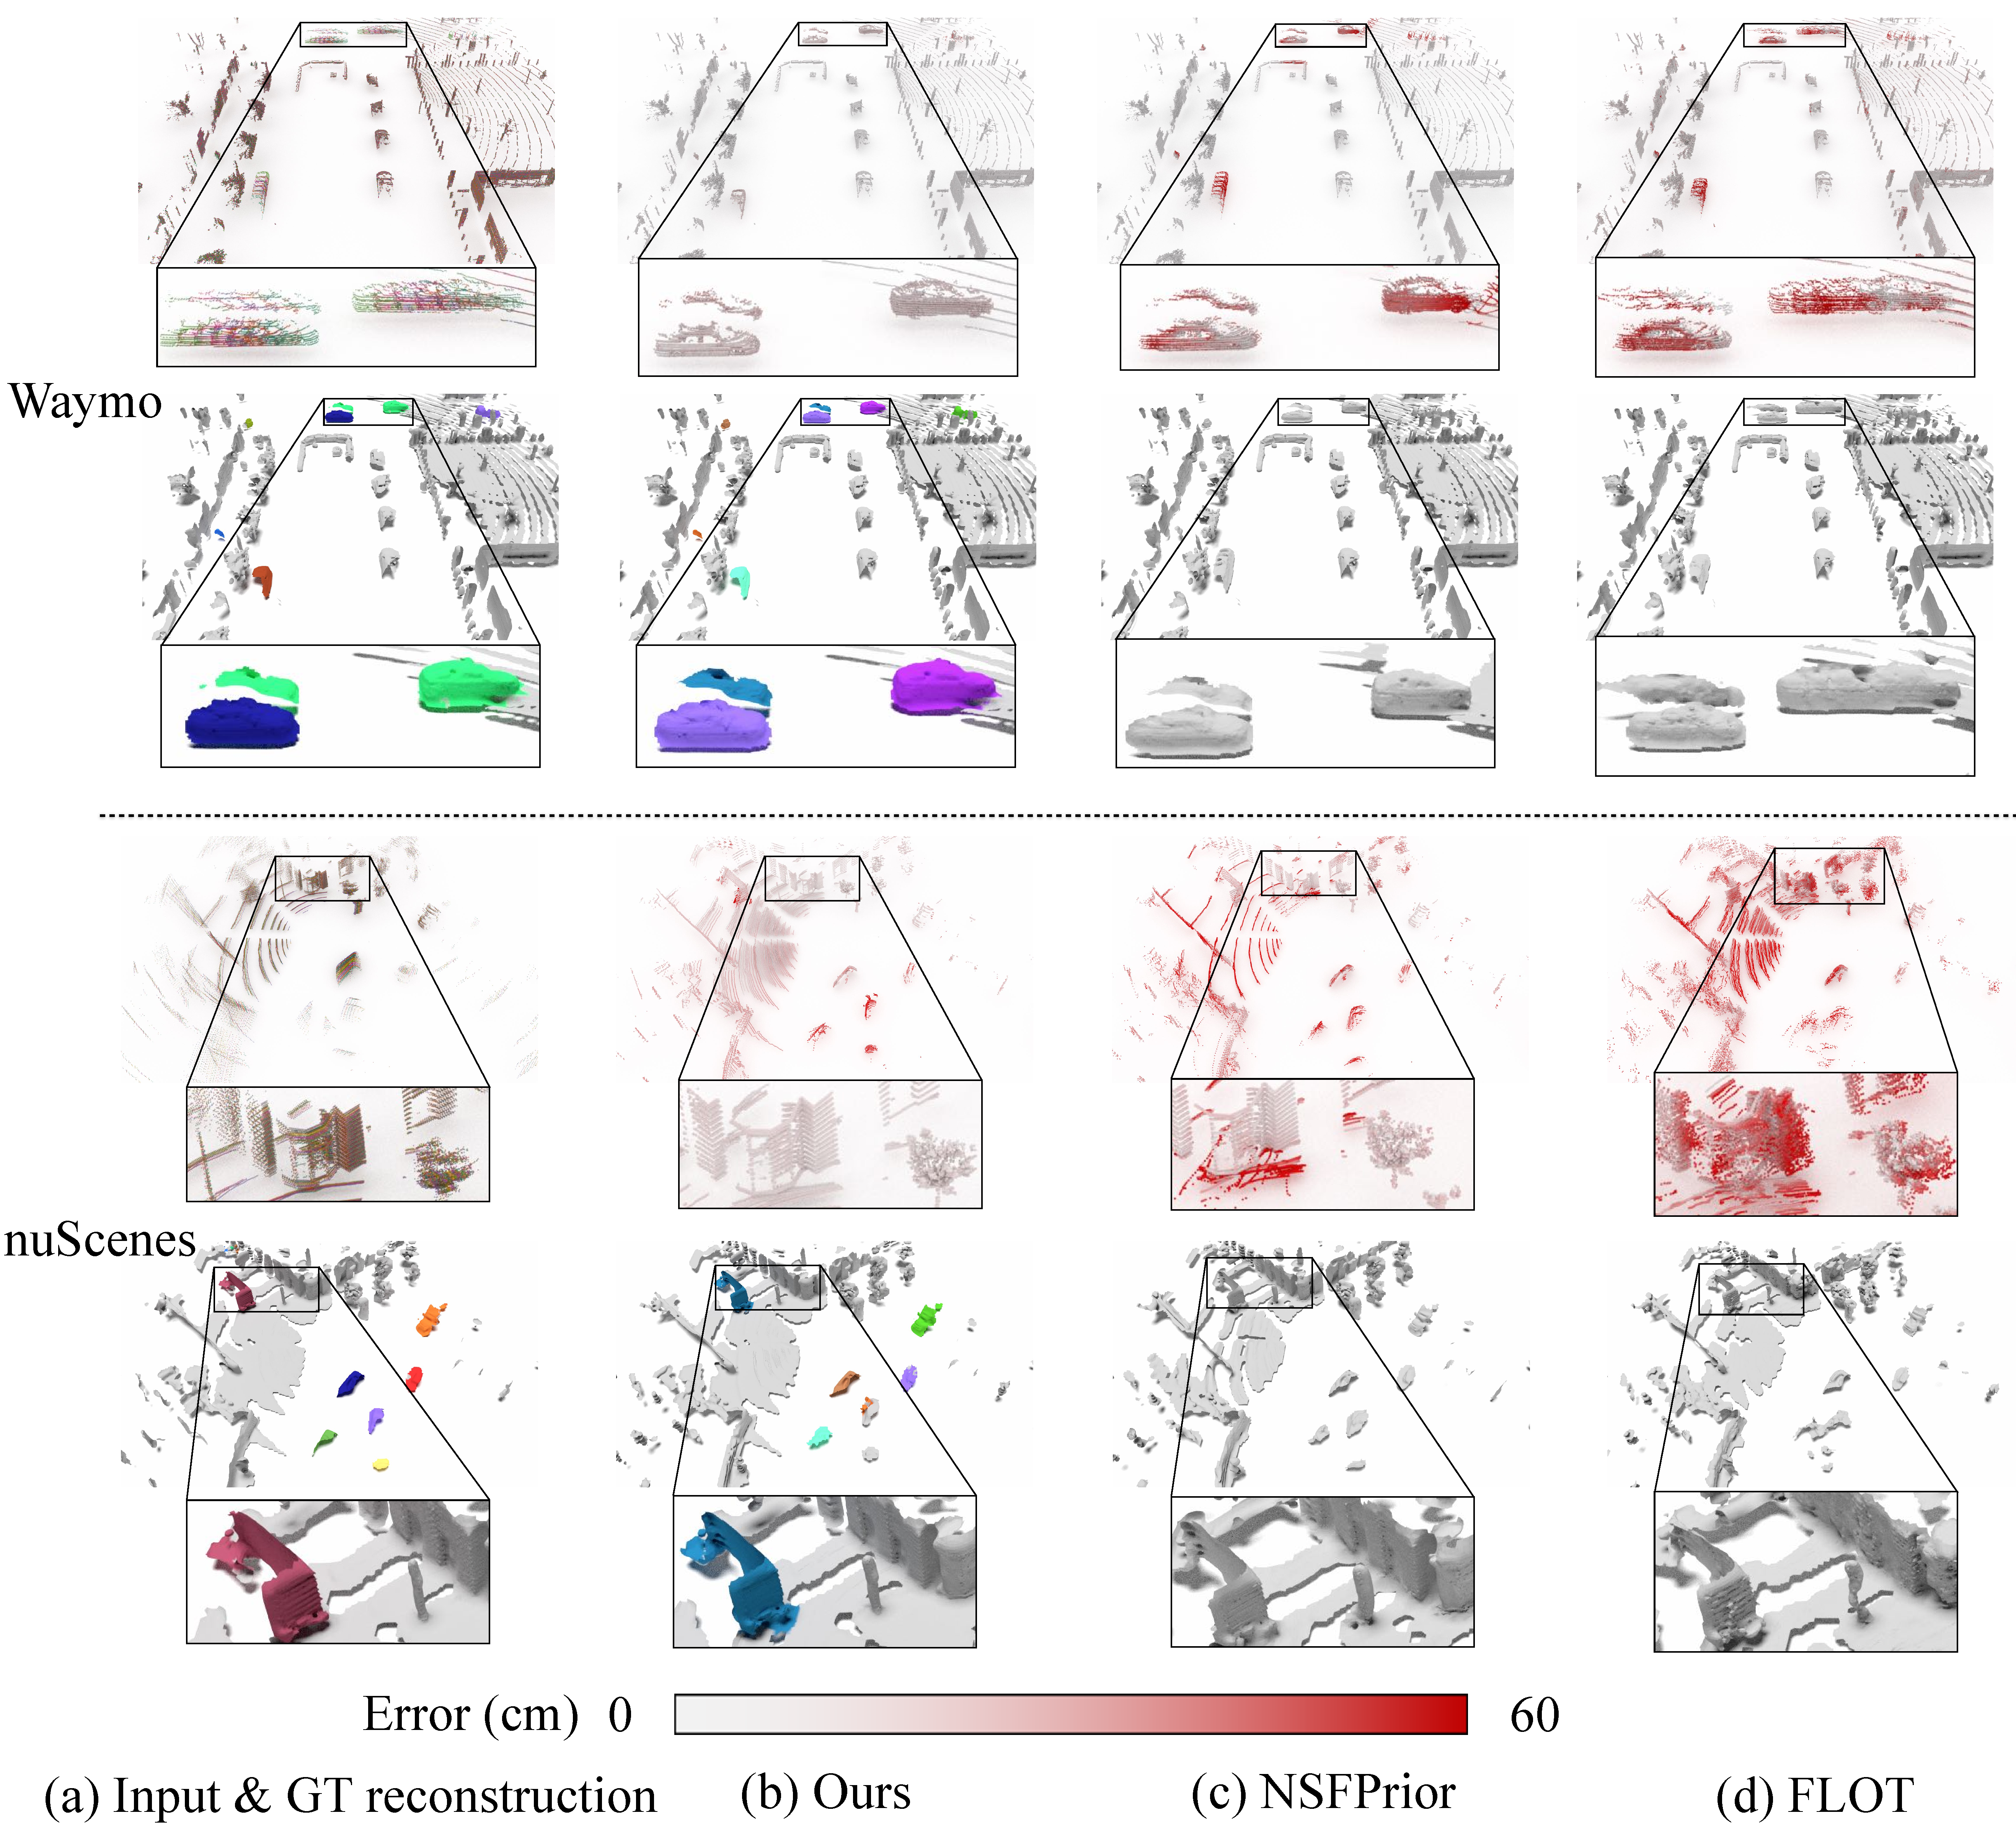
\includegraphics[width=0.88\columnwidth]{figs/figure/main_vis.pdf}
    \caption{Qualitative results showing scene flow estimation (top) and surface reconstruction (bottom) for two example scenes from \waymo~and \nuscenes.}
    \label{fig:qualitative_results}
\end{figure}
In~\cref{fig:qualitative_results} we show qualitative examples of scene and object reconstruction with our approach. By jointly estimating the ego-motion of the static part and the moving object motions, our method accumulates the corresponding points into a common, motion-compensated frame. It thus provides an excellent basis for 3D surface reconstruction.


\begin{table}[t]
    \setlength{\tabcolsep}{6pt}
    \renewcommand{\arraystretch}{1.2}
    \centering	
    \resizebox{\columnwidth}{!}{
    \begin{tabular}{cccc|cc|c|c|c|ccccc}
    \toprule
      & \multicolumn{3}{c|}{Modules} & \multicolumn{2}{c|}{Motion seg.} & \multicolumn{1}{c|}{Association} &\multicolumn{1}{c|}{Static BG} &  \multicolumn{1}{c|}{Static FG} &  \multicolumn{5}{c}{Dynamic FG} \\
    & FG & MOS & Offset & recall$\uparrow$ & precision$\uparrow$ & WCov$\uparrow$ & EPE avg.$\downarrow$ & EPE avg.$\downarrow$ & EPE avg.$\downarrow$ & EPE med.$\downarrow$ & AccS$\uparrow$ & AccR$\uparrow$ & ROutliers$\downarrow$   \\
    \midrule
    \multirow{4}{*}{\emph{Waymo}} & & \ding{51} & \ding{51} & \underline{92.7} & 94.6 & 82.2 & 0.041 & 0.028 & 0.286 & 0.071 & 45.5 & 71.3 & 10.8\\
    & \ding{51} & & \ding{51} & - & - & \textbf{83.0} & 0.031 & 0.190 & 0.198 & 0.062 & \textbf{53.5} & 77.4 & 6.3\\
    & \ding{51} & \ding{51} & & 92.2 & 96.5 & 79.1 & 0.029 & 0.021 & 0.202 & 0.064  & 52.5 & 76.1 & 6.1\\
    & \ding{51} & \ding{51} & \ding{51} & 92.2 & \textbf{96.8} & 80.4 & \textbf{0.029} & \textbf{0.021} & 0.197 & \textbf{0.062} & 53.3 & \textbf{77.5} & 5.9 \\
    \arrayrulecolor{lightgray}\cline{2-14}\arrayrulecolor{black}
    \multirow{4}{*}{\emph{nuScenes}} & & \ding{51} & \ding{51} & 87.8 & \textbf{92.5} & 65.1 & 0.115 & 0.076 & 0.333 & 0.153 & 25.0 & 50.9 & 13.8\\
    & \ding{51} & & \ding{51} & - & - & \textbf{66.8} & 0.118 & 0.199 & \textbf{0.296} & \textbf{0.143} & \textbf{26.9} & \textbf{53.9} & \textbf{11.7}\\
    & \ding{51} & \ding{51} & & 89.2 & 90.7 & 60.2 & \textbf{0.113} & 0.075 & 0.348 & 0.149 & 25.8 & 51.9 & 13.9 \\
    & \ding{51} & \ding{51} & \ding{51} & \textbf{89.3} & 90.8 & 63.2 & 0.114 & \textbf{0.074} & 0.301 & 0.146 & 26.6 & 53.4 & 12.1\\
    \midrule
    \multirow{2}{*}{\emph{Waymo}} & \multicolumn{3}{c|}{Kalman tracker} & 92.3 & 96.6 & 77.1 & 0.030 & 0.027 & 0.586 & 0.099 & 36.3 & 61.6 & 11.7 \\
    & \multicolumn{3}{c|}{chained poses} & \textbf{93.2} & 94.9 & 81.9 & 0.044 & 0.030 & \textbf{0.171} & 0.068 & 48.0 & 77.0  & \textbf{4.8}\\
    \arrayrulecolor{lightgray}\cline{2-14}\arrayrulecolor{black}
    \multirow{2}{*}{\emph{nuScenes}} & \multicolumn{3}{c|}{Kalman tracker} & 89.4 & 90.8 & 42.9 & 0.114 & 0.092 & 1.238 & 0.364 & 10.7 & 25.1 & 44.0 \\
    & \multicolumn{3}{c|}{chained poses} & 88.1 & 90.2 & 62.1 & 0.225 & 0.151 & 0.315 & 0.155 & 23.4 & 51.8 & 13.4\\
    \bottomrule
    \end{tabular}
    } 
    \caption{Ablation studies on \emph{Waymo} and \emph{nuScenes} datasets.} 
    \label{tab:ablations}
\end{table}



% \begin{table}[t]
%   \setlength{\tabcolsep}{6pt}
%   \renewcommand{\arraystretch}{1.2}
%   \centering	
%   \begin{tabularx}{\textwidth}{YYYY|YY|Y|Y|Y|YYYYY}
%   \toprule
%     & \multicolumn{3}{c|}{Modules} & \multicolumn{2}{c|}{Motion seg.} & \multicolumn{1}{c|}{Association} &\multicolumn{1}{c|}{Static BG} &  \multicolumn{1}{c|}{Static FG} &  \multicolumn{5}{c}{Dynamic FG} \\
%   & FG & MOS & Offset & recall$\uparrow$ & precision$\uparrow$ & WCov$\uparrow$ & EPE avg.$\downarrow$ & EPE avg.$\downarrow$ & EPE avg.$\downarrow$ & EPE med.$\downarrow$ & AccS$\uparrow$ & AccR$\uparrow$ & ROutliers$\downarrow$   \\
%   \midrule
%   \multirow{4}{*}{\emph{Waymo}} & & \ding{51} & \ding{51} & \underline{92.7} & 94.6 & 82.2 & 0.041 & 0.028 & 0.286 & 0.071 & 45.5 & 71.3 & 10.8\\
%   & \ding{51} & & \ding{51} & - & - & \textbf{83.0} & 0.031 & 0.190 & 0.198 & 0.062 & \textbf{53.5} & 77.4 & 6.3\\
%   & \ding{51} & \ding{51} & & 92.2 & 96.5 & 79.1 & 0.029 & 0.021 & 0.202 & 0.064  & 52.5 & 76.1 & 6.1\\
%   & \ding{51} & \ding{51} & \ding{51} & 92.2 & \textbf{96.8} & 80.4 & \textbf{0.029} & \textbf{0.021} & 0.197 & \textbf{0.062} & 53.3 & \textbf{77.5} & 5.9 \\
%   \arrayrulecolor{lightgray}\cline{2-14}\arrayrulecolor{black}
%   \multirow{4}{*}{\emph{nuScenes}} & & \ding{51} & \ding{51} & 87.8 & \textbf{92.5} & 65.1 & 0.115 & 0.076 & 0.333 & 0.153 & 25.0 & 50.9 & 13.8\\
%   & \ding{51} & & \ding{51} & - & - & \textbf{66.8} & 0.118 & 0.199 & \textbf{0.296} & \textbf{0.143} & \textbf{26.9} & \textbf{53.9} & \textbf{11.7}\\
%   & \ding{51} & \ding{51} & & 89.2 & 90.7 & 60.2 & \textbf{0.113} & 0.075 & 0.348 & 0.149 & 25.8 & 51.9 & 13.9 \\
%   & \ding{51} & \ding{51} & \ding{51} & \textbf{89.3} & 90.8 & 63.2 & 0.114 & \textbf{0.074} & 0.301 & 0.146 & 26.6 & 53.4 & 12.1\\
%   \midrule
%   \multirow{2}{*}{\emph{Waymo}} & \multicolumn{3}{c|}{Kalman tracker} & 92.3 & 96.6 & 77.1 & 0.030 & 0.027 & 0.586 & 0.099 & 36.3 & 61.6 & 11.7 \\
%   & \multicolumn{3}{c|}{chained poses} & \textbf{93.2} & 94.9 & 81.9 & 0.044 & 0.030 & \textbf{0.171} & 0.068 & 48.0 & 77.0  & \textbf{4.8}\\
%   \arrayrulecolor{lightgray}\cline{2-14}\arrayrulecolor{black}
%   \multirow{2}{*}{\emph{nuScenes}} & \multicolumn{3}{c|}{Kalman tracker} & 89.4 & 90.8 & 42.9 & 0.114 & 0.092 & 1.238 & 0.364 & 10.7 & 25.1 & 44.0 \\
%   & \multicolumn{3}{c|}{chained poses} & 88.1 & 90.2 & 62.1 & 0.225 & 0.151 & 0.315 & 0.155 & 23.4 & 51.8 & 13.4\\
%   \bottomrule
%   \end{tabularx}
%   \caption{Ablation studies on \emph{Waymo} and \emph{nuScenes} datasets.} 
%   \label{tab:ablations}
% \end{table}
\subsection{Ablation Study}
\label{sec:ablation}
\paragraph{Sequential model}
We evaluate the individual modules of our sequential model, namely the foreground segmentation (\textit{FG}), motion segmentation (\textit{MOS}) and offset compensation (\textit{Offset}). We train two models with and without foreground segmentation. For variants without \textit{MOS} or \textit{Offset}, we take the trained full model but remove \textit{MOS} or \textit{Offset} at inference time. The detailed results are summarised in \cref{tab:ablations}. \textit{FG} enables us to exclude dynamic foreground objects during pairwise registration. On \waymo, this reduces EPE of the static parts by $30\%$ from 4.1 to 2.9$\,$cm, and as a result also reduces EPE of dynamic parts from 28.6 to 19.7$\,$cm. By additionally extracting the static foreground parts with \textit{MOS}, the model can recover more accurate ego-motion for them, which reduces EPE from 19.0/19.9 to 2.1/7.4$\,$cm on \waymo/\nuscenes. \textit{Offset} robustifies the instance association against low point density and fast object motion (+3.1 $pp$ in \textit{WCov} on \nuscenes), this further reduces the EPE of dynamic parts by 3.7$\,$cm. 

\paragraph{Ego-motion estimation strategy}
By default, we directly estimate the ego-motion from any \textit{source} frame to the \textit{target} frame. We compare to an alternative which estimates the ego-motion relative to the previous frame. Although that achieves smaller pairwise errors, after chaining the estimated poses the errors w.r.t.\ the \textit{target} frame explode, resulting in inferior scene flow estimates (\textit{chained poses} in \cref{tab:ablations}).

\paragraph{Comparison to tracking-based method}
Instead of running spatio-temporal association followed by TubeNet to model the motion of each moving object, an alternative would be to apply Kalman tracker so as to simultaneously solve association and motion. We compare to the modified AB3DMOT~\cite{weng20203d}, which is based on a constant velocity model. That method first clusters moving points for each frame independently to obtain instances, then associates instances by greedy matching of instance centroids based on $L_2$ distances. The results in \cref{tab:ablations} (\textit{Kalman tracker}) show clearly weaker performance, due to the less robust proximity metric based on distances between noisy centroid estimates. 